
\section{Plasma Wakefield Acceleration}

Current RF accelerator technology is limited to an electromagnetic gradient of
about \SI{100}{\mega\electronvolt\per\meter} due to material breakdown in the
walls of the structure.  The ability of plasma to sustain very large
electromagnetic fields makes it a good candidate for a medium within which
charged particles can be accelerated. The concept being that the plasma can act
as an energy transfer medium, removing energy from a driver beam, such as a
laser or a proton beam, and transferring it to a bunch of charged leptons.  As
the driver beam travels through the plasma cell, it leaves an oscillating
electromagnetic field in it's wake. The beam to be accelerated (the witness
beam) is injected ahead of a propagating electromagnetic field as shown in
Figure~\ref{fig:phase-b} where it is accelerated under the electromagnetic
gradient.  In 1979, the concept of laser plasma acceleration was shown in
simulations to be of practical use in accelerators and
pulsers~\cite{Tajima:1979bn}. More recently, proof-of-concept experiments
implementing laser plasma acceleration have been shown to accelerate electrons
to the \si{\giga\electronvolt} scale in a \si{\centi\metre}-scale plasma
cell~\cite{Lu:2006nz,Leemans:2006dx}, providing results that are consistent with
simulations.


\subsection{The AWAKE Project}

Simulations of plasma wakefield accelerators driven by proton beams were
carried out in \num{2009}~\cite{Caldwell2008ak}, showed the high energy transfer
efficiency between a driver proton bunch and an electron witness bunch. In these
simulations, a \SI{1}{\tera\electronvolt} proton beam drove the wakefield in a
\SI{400}{\meter} long plasma cell, which accelerated a
\SI{10}{\giga\electronvolt} electron beam to \SI{650}{\giga\electronvolt}.  The
AWAKE project is a proof-of-concept experiment for proton driven plasma
wakefield acceleration with the goal of accelerating \SI{15}{\mega\electronvolt}
electrons up to \SI{\sim1.3}{\giga\electronvolt} over a distance of
\SI{10}{\meter}. Later, aiming to reach \SI{10}{\giga\electronvolt} in the same
distance. This will demonstate the use of electromagnetic gradients that are
about 10 times larger than current RF acceleratrs.

A few challenges arose in the design of this experiment and are discussed next.


\subsubsection{Proton Bunch Length}

The first challenge in the development of this accelerator was getting the
length of the proton driver bunch small enough such that it is able to create
resonant waves in the plasma. Typical proton bunches such as those produced by
the CERN Super Proton Synchrotron (SPS), have lengths of \(\sim
\SI{10}{\centi\meter}\) which alone, cannot create strong plasma waves at the
required wavelength in the \si{\milli\meter} scale as the Fourier component of
the proton beam at the plasma frequency is negligible.
Simulations~\cite{kumar2010self} on the compression of these proton bunches to
such small distances, show that
reducing the longitudinal phase volume blows up the transverse phase volume,
resulting in a diverging beam with a large emittance. % TODO is this correct?
An alternative method would be to split up the proton bunch into a number of
micro-bunches to be simultaneously decelerated, all of which contribute energy
to the wakefield.

The splitting of the proton beam can be achieved by using an instability
between the beam and the plasma arises from the mutual
amplification of the rippling of the beam radius and the plasma wave, known as
self-modulated instability (SMI). This
instability tends to destroy the plasma wave as the amplification focuses and
defocuses various parts of the beam. 
% This problem was solved
However, by seeding the SMI with a short electron bunch~\cite{lotov2013natural},
a laser pulse~\cite{siemon2013laser} or a sharp cut in the bunch
profile~\cite{kumar2010self}, a single mode of the oscillating plasma wave and
beam rippling will be promoted while others will be suppressed. This produces
% including the strongest
% competing modes, the hosing modes
% \cite{vieira2014hosing} and produce
well-separated micro-bunches of protons with of a short enough length to induce
a plasma wave at the resonance frequency of the plasma.  The plasma wavelength
is \(\lambda_{pe} \approx \SI{1.26}{\milli\meter}\) meaning that the
\SI{10}{\centi\meter} proton bunch will have to be split into \(\sim 100\)
micro-bunches in order to be able to drive the wake. 


\subsubsection{Uniform-Density Plasma Cell}

\begin{figure}[!tb]
	\centering
	\begin{subfigure}{\linewidth}
		\centering
		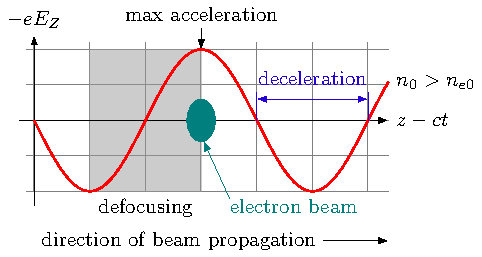
\includegraphics[width=\textwidth]{figures/phases-a.pdf}
		\caption{Injection of the electrons for a shorter plasma wavelength,
		where electrons may crest the wave.}
		% \caption{Injection at the peak of a wave will allow parts of the
		% electron to fall into the defocusing region of the wave.}
		\label{fig:phase-a}
	\end{subfigure}
	\begin{subfigure}{\linewidth}
		\centering
		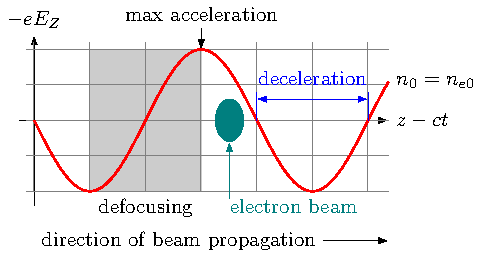
\includegraphics[width=\textwidth]{figures/phases-b.pdf}
		\caption{Injecting at the ideal phase, where all electrons will be
		accelerated.}
		\label{fig:phase-b}
	\end{subfigure}
	\begin{subfigure}{\linewidth}
		\centering
		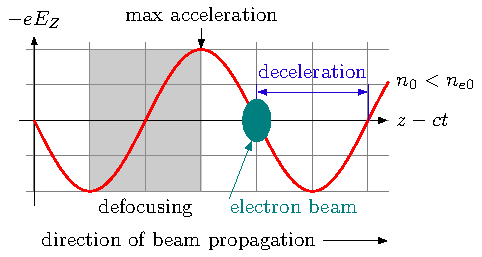
\includegraphics[width=\textwidth]{figures/phases-c.pdf}
		\caption{Injection for a longer plasma wavelength, where electrons may
		fall into the deceleration region.}
		\label{fig:phase-c}
	\end{subfigure}
	\caption{
		Phase of the injection of the electron
		beam~\cite{wiedemann2007particle}.
		% Phasing of the electron bunch for increased density (a) correct density
		% (b) and decreased density (c).
	}
	\label{fig:phases}
\end{figure}


All proton micro-bunches contribute to the wakefield, and only if the plasma
density is uniform, will the contribution of each bunch be coherent. Incoherent
proton bunches
will cause alterations in the plasma wakefield meaning the electron bunches
arrive at the wrong phase of the plasma
oscillation. An increase in the plasma density will shorten the plasma
wavelength causing the electron bunch to crest plasma wave it was riding and
fall into the defocusing phase of the plasma wave as shown in
Figure~\ref{fig:phase-a}. A decrease in the plasma density will increase the
plasma wavelength causing the plasma wave to fall further behind the electron
bunch meaning the electron bunch to fall into the trough of the plasma wave
resulting in a deceleration of the electron beam \ref{fig:phase-c}. The electron
beam must be in the region of length \(\lambda_{pe}/4\) between the defocusing
and decelerating phases of the plasma wave in order to be appropriately
accelerated. These effects also affect the proton beam, however due to their
large longitudinal momentum these effects are significantly larger for the
electrons.

This requirement of the plasma limits the plasma selection to being uniform
rubidium vapor, ionised by a co-propagating laser pulse \cite{oz2014novel,
oz2014bja}. Rubidium was chosen due to it's low ionization potential and heavy
atomic mass. A heavy element is required to minimize the movement of the
plasma's nuclei which causes adverse effects on the plasma's behaviour
\cite{vieira2012nj,vieira2014bqa}. The Rubiduim vapor is kept in thermodynamic
equilibrium at a constant temperature and volume.


\subsubsection{Injection of the Witness Beam}

% TODO citations
Due to SMI, the shape of the drive beam changes in the plasma and for the first
four meters, the difference between the phase velocity of the wakefield and the
proton beam velocity is quite large and this will effect the electron beam in
the same manner as having a non uniform plasma, detailed above. To avoid this
problem it was suggested that the electrons could be injected into the plasma
after SMI had fully developed. The design of the injection method arrived at
passing the electron beam through a narrow vacuum tube separated from the
plasma by a thin foil. Then after \(\sim \SI{4}{\meter}\) the electrons will be
directed into the wakefield close close behind the proton driving beam.

\subsubsection{AWAKE Overview}

The SPS will provide a \SI{400}{\giga\electronvolt} proton beam with a bunch
length of \(\sigma_z = \SI{12}{\centi\meter}\) and an intensity of \(\sim
\num{3e11}\) protons per bunch. This will travel down the \SI{750}{\meter} long
proton beam line, previously used for the CERN Neutrinos to Gran Sasso project
(CNGS), and will be focused infront of the plasma cell to a horizontal and
vertical beam size of \(\sigma_{x,y} = \SI{200}{\micro\meter}\). This beam will
then enter the \SI{10}{\meter} long Rubiduim vapor plasma cell with an
adjustable density at the \num{e14} to \num{e15} \si{electrons\per\centi\meter}
scale.

The proton driver will self modulate at the plasma wavelength \(\lambda_{pe}\)
after being seeded by a high powered \(\approx \SI{4.5}{\tera\watt}\) laser
pulse that is co-axial and co-propagating with the proton driver beam. This
laser also serves the purpose of ionising the Rubidium vapor to create the
plasma. For these beams to be co-axial for the full length of the plasma cell,
they need to be synchronous to within \SI{100}{\pico\second} and the size of the
focal point of the proton beam is required to be \(\le\SI{100}{\micro\meter}\)
and \(\le\SI{15}{\micro\radian}\)

% TODO cite 
The electron witness beam will be created via photo-emission by an illuminating
cathode electron source. It will then be accelerated by a 2.5 cell RF-gun and a
meter long booster at both at \SI{3}{\giga\hertz}.  This will accelerate the
beam up to \SI{20}{\mega\electronvolt} and an energy spread of
\SI{0.5}{\percent}.
% !! TODO describe electron and laser beamlines


% \section{Project outline}

% \lipsum[3-10]

% The development of this experiment has been heavily simulation driven.
% Simulation code developed specifically for the simulation of the plasma to be
% able to resolve for time scales of \(\omega_p^{-1}\), (where \(\omega\) is the
% frequency of the plasma wave) and length scales of down to \(c/\omega_p\), as
% existing codes were not tuned to resolve at these scales.  Different simulation
% softwares are tuned to be used for different sections of the AWAKE experiment.

% I will be working on simulating the electron spectrometer using
% BSDIM~\cite{agapov2009bdsim}, simulation software in active development,
% designed to simulate and track particle beams passing through accelerators and
% detectors. It is built on top of the Geant4
% toolkit~\cite{agostinelli2003geant4} for the simulation of particles through
% matter, which also provides the graphical user interface for a visualisation of
% the simulation.  Event data is stored using ROOT~\cite{antcheva2011root}, an
% advanced statistical analysis and visualisation framework designed to work for
% petabyte scale data storage.

% More specifically, I will initially be looking at calculating the emittance of
% the accelerated electron beam using data from simulated accelerated electron
% beams.  Recent simulations of the spectrometer used an idealised electron beam
% \cite{deacon2016qjq} and I will be continuing this line of investigation.  The
% electron beam profile and other properties immediately after it leaves the
% plasma cell will be provided by separate simulations using LCODE.  This data is
% used as input for the BDSIM simulation where we will simulate the beam passing
% through dual focusing quadrupoles in both the horizontal and vertical planes.
% The simulation will be able to provide all the raw data about the final state
% of the electron beam, however, in reality we will not be able to simply query
% the beam properties. The measurement of the energy spectrum will be carried out
% by using a magnetic dipole downstream of the dual quadrupoles, and observing
% the horizontal spread of the electron beam on a screen. This screen will also
% be sumulated with BDSIM taking into account the screen resolution and detection
% rates.

% I will also be working on the modeling and simulation of the background
% radiation from the plasma cell and other sources using real world data to help
% build an accurate model.  All of these simultions along with real data will
% help in finding optimal parameters for each component of the spectrometer,
% including the strength of the quadrupoles and the dipole, the lens parameters
% of the camera and the properties of the screen.

